\Chapter{Represenation of plot state using a agent-based simulation}

\section{Agents and architecture}

Both the player and any non-playable characters can be called agents.
Each agent is independent from the rest and is able to act based on the subset of the plot available to them.
The actual implementation of each agent's behaviour can be as simple as a hardcoded line of dialogue and as complex as a set of rules enabling emergent behaviour.
General plot of the game as experienced by the player is the sum of interactions and sub-plots of the individual agents in the game.
Grey et al.\cite{grey2011procedural} proposed a solution using agent-based simulation to create procedural quests.
This work focuses on extension of the original approach using a SOAR cognitive architecture\cite{rosenbloom1993soar}.

\subsection{SOAR}

One of the most important developments in the area of multi-agent systems and cognitive modelling was the SOAR (State, Operator, And Representation) cognitive architecture \cite{laird2019soar}.
It is a cognitive architecture that is designed to simulate human thinking and problem-solving processes.
At its core, SOAR is a symbolic, production-based system that uses rules to guide behavior.
This architecture consists of two major components:

\begin{itemize}
    \item Procedural memory (production memory) - set of production rules that take working memory elements and propose operators (behaviours) or modify the state of working memory (inferences)
    \item Working memory - fact based knowledge represented by a symbolic graph structure describing the current state of the world
\end{itemize}

Many implementations of this architecture additionally include the concept of long-term memory structure that accumulates knowledge during the whole lifetime of the agent.
In general, implementation of the SOAR architecture can be called a production system.
Unlike many traditional production systems however, all rules that match against the current state of the world will fire (execute actions) in parallel.
This means that the list of rules is not ordered and conflicting operators may be proposed.
In such cases the usual strategy is to create a substate of the working memory with a new goal of conflict resolution.

The SOAR architecture has been successfuly utilized in creation of video game AI agents.
Examples include the application of this architecture to create an autonomous agent designed for playing Quake\cite{laird2001knows}, StarCraft\cite{turner2013soar-sc} and Descent 3\cite{van1999developing}.
Michael van Lent and John Laird in their work "Developing an Artificial Intelligence Engine"\cite{van1999developing} describe a decision cycle in an inference machine:

\begin{itemize}
    \item Perceive: Accept sensor information from the game
    \item Think: Select and execute relevant knowledge
    \item Act: Execute actions in the game
\end{itemize}

This cycle combined with the SOAR architecture allows for creation of a versatile agent capable of processing and propagating plot events in the game.
The first step allows the agent to modify the state of the working memory.
It can detect visible objects, including other agents and interactables such as containers, doors or even writings.
The second step is divided into two substeps, the first executes inference rules and modfies the state of the working memory while the other part executes behaviour rules which propose operators.
Operators modify the state of the world, for example by moving the agent, taking the contents of a container, opening doors or interacting with another agent.
This constitutes the last step of the cycle and allows the agent to go back to the first step and update its working memory in preparation for the next step.

This architecture is versatile in that it can be used to model even very complex behaviours.
In order to avoid conflicts in the proposed operators by production rules that try to solve different goals, a goal token can be inserted into the working memory and used as a dependency in the production rules.
This way an agent may have a rule that changes the goal of the agent and thus modifies its next sequence of actions.
The general model of an agent can be seen on figure \ref{fig:agent.drawio.png}.

\begin{figure}[h]
    \centering
    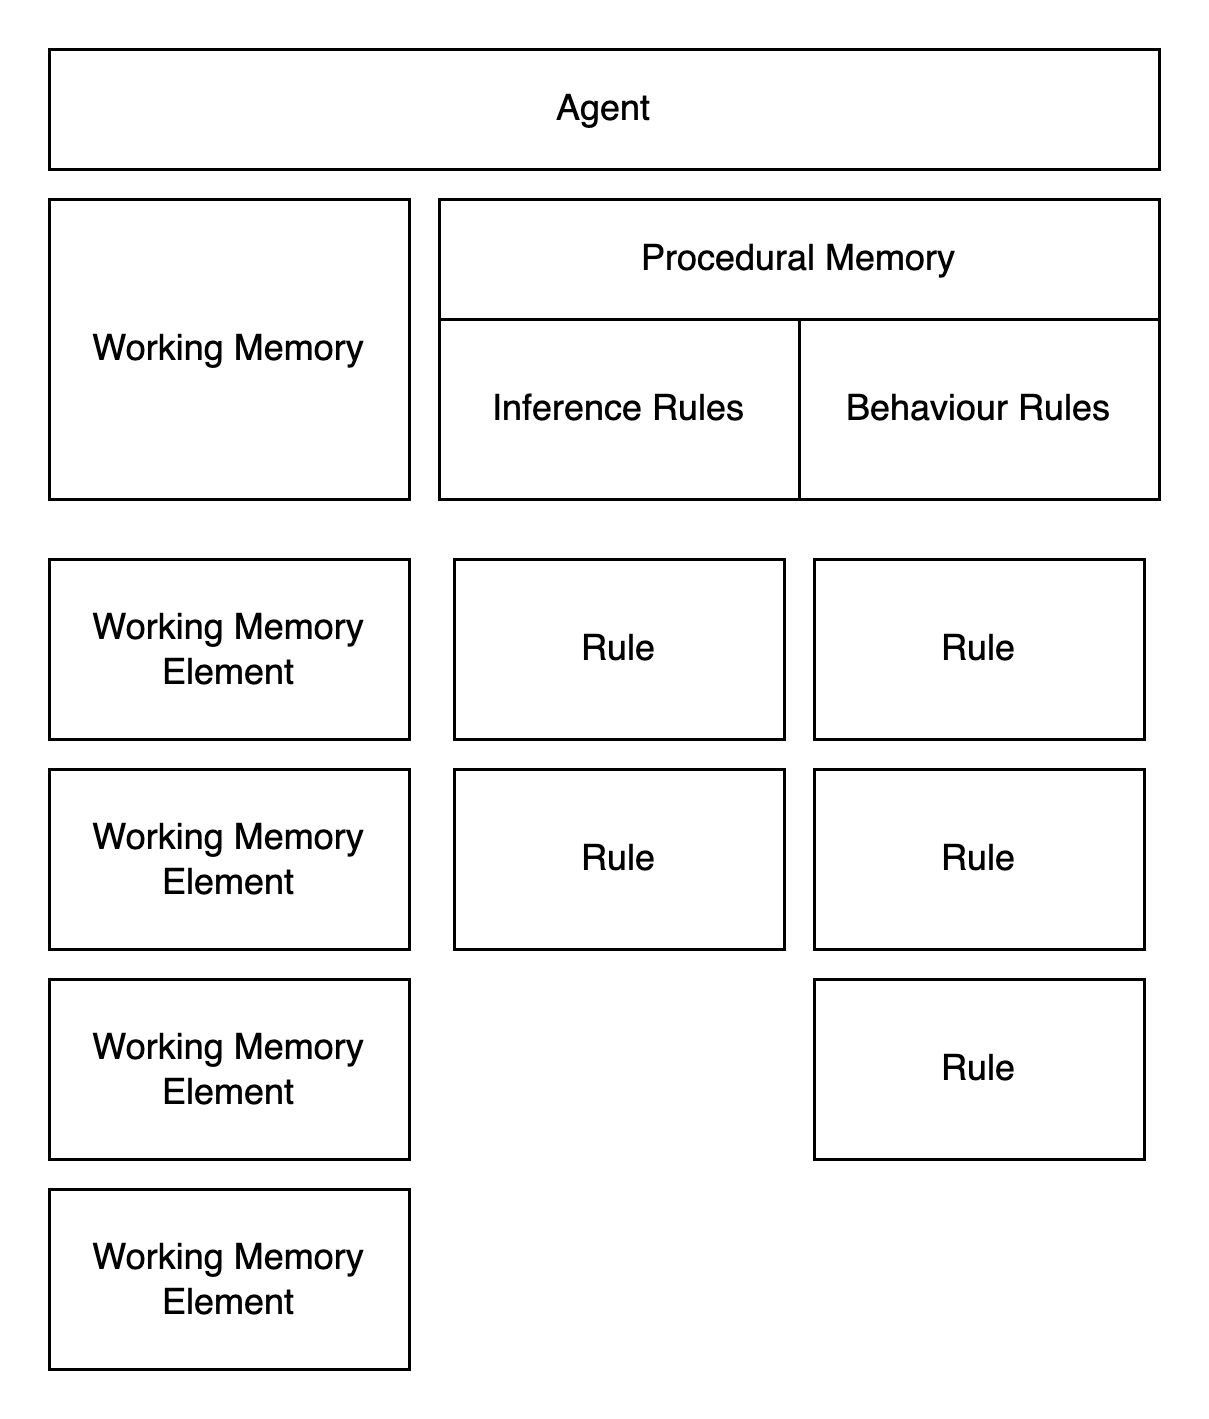
\includegraphics[width=0.6\textwidth]{images/chapter1/agent.drawio.png}
    \caption{Conceptual model of an agent}\label{fig:agent.drawio.png}
\end{figure}

\subsection{Perceive}

The agent is equipped with simulated sensors that feed into its working memory.
These sensors interact with the simulated world and process the description of the world producing information that is then stored in the working memory of the agent.
Sensory information might include sight, hearing, sense of smell and other commonly thought of senses as well as abstract and arbitrary information that the agent can somehow perceive.
The combined information from all the sensors might produce information regarding the agent's awareness of the vicinity and the location of other agents in the simulated system as well as the state of the agent's body and own position in the game world.
The information is presented to the agent and it is up to the agent to decide what to do with it.
Sensors may only influence working memory of the agent.

\subsection{Think}

Agents have procedural memory that is represented by a collection of production rules that are executed in parallel.
Procedural memory is divided into inference rules and behaviour rules.
The first kind of memory elements are production rules that adjust the working memory of the agent before taking action.
The inference rules are evaluated sequentially in an undefined order and mutate the state of the working memory.
For this reason, it is essential that the designer of the agent ensures no conflicting inference rules are present.
Otherwise undefined behaviour might occurr, usually causing a rule to override the effects of another rule.
Behaviour rules do not modify the state of the working memory but instead produce operators that are used to evaluate the action the agent wishes to perform.
Each rule might take as input an arbitrary set of working memory elements (WME), check arbitrary preconditions and produce arbitrary operators that when evaluated will change the state of the simulated world by means the agent's action.
While working memory is perfect for storing the immediate description of the agent's state, it is perhaps ill suited for storage of event based information elements.
For this reason the notion of long term memory is used for storage of facts characterized by timestamp of occurrence and description of the event.
Procedural memory and production rules therein may also utilize this storage to work with temporal data, for example to facilitate the agent remembering its travel trajectory or recording events such as successful executions of certain actions.
Procedural memory is usually immutable after creation of the agent but it is possible to store a production rule inside of working memory and by means of another production rule, modify the procedural memory adding the new rule to the bank of rules the agent possesses.
This can simulate agent learning new inference rules and behaviours, for example through reading a book or being taught by other agent.

\subsection{Act}

The act of action when performed by the simulated agent is represented by an operator being evaluated.
An operator represents an action that an agent wishes to perform.
The game world is in charge of evaluating the results of the operator and rejecting it in case the agent is not allowed to perform it due to any condition that the agent itself is not aware of.
Because production rules are executed in parallel and thus output multiple operators, it is possible for conflicts to occur.
A single agent may think to move forward and back at the same time.
Because the order in which actions are performed may impact the result, it is important to define a conflict resolution strategy, either for each agent or for the whole game in general.
Such a strategy does not need to necessarily be deterministic as usually it is impossible to determine which operator should take precedence and defining conflict resolution policies for each possible set of conflicting operators is often not a viable approach.
One example of a conflict resolution strategy is a strategy that chooses a random order for conflicting operators and executes them until one is accepted.
This shows the second part of the problem which is conflict detection.
Any two operators can be conflicting in terms of resulting state of the game world.
The simplest approach is not allowing the agent to execute multiple operators at the same time and instead force it to choose one specific action instead.

\subsection{Interactions}

An agent might lack the sense of vision and instead start with its known position WME at coordinates $v_0=(0, 0)$.
It wishes to progress forward (positive $y$ axis) and so proposes the operator $Move(Agent, 0, 1)$ via a production rule with constant output.
The game world accepts the operator, evaluates it and the agent is then made aware of the operator's successful execution.
The agent now has the position WME set to $v=(0, 1)$.
It proposes the same operator again.
This time the game world rejects the action because of a wall that stands at $v=(0, 2)$.
The agent did not modify its position WME this time but added a second WME $WallAt(0, 2)$.
A production rule exists that checks if there is a $WallAt$ WME directly ahead of the current position and if so, produces operator $Move(Agent, 1, 0)$.
The production rule that produces the constant $Move(Agent, 0, 1)$ operator fires as well and afterwards the agent needs to decide which action to take.
The agent has a conflict resolution strategy defined as:

\begin{itemize}
    \item choose random
    \item fallback when action rejected
\end{itemize}

This policy means that either the lateral move will be selected by random chance or the previous operator will be selected, evaluated, subsequently rejected and a fallback would occurr to the next one.
This example shows that a virtual agent possesses a limited capacity to learn and build the information bank describing the state of the world around it.
In some implementations, the immediate position of the agent would be stored as WME while the position of each discovered wall would be put in long-term memory.

\subsection{Simulation constraints and limitations}

The simulatated environment presented in this work was designed to resemble the environment described by Grey et al.\cite{grey2011procedural} which in turn used the implementation done by Prageeth Silva\cite{silva2010shadow}.
As of the time of writing, the original implementation of Shadow Quest used in evaluation of Grey's model is unavailable and so a custom implementation with modifications was made specifically for the sake of experimentation.
Each agent may occupy a single tile in a grid-based world.
The temporal structure used in the design of the simulation is based on the concept of turns.
Because the interaction with a human player is not necessary to simulate the progression of a procedurally emergent plot, the turns are simply simulatin steps.
Within a single turn all agents execute the aforementioned decision cycle, starting from receiving information regarding the state of the world around them, deciding on the action to perform and finally executing it.
The simulation used for evaluation of the model presented in this work is limited to a set of actions that each agent may perform.

\begin{itemize}
    \item Idle - agent does nothing, stays idle for the whole turn
    \item Move - agent may decide to move in one of the four cardinal directions by a single tile
    \item Attack - agent attacks another agent
    \item Interact - agent interacts with something such as another agent or world entity
\end{itemize}

Because all agents execute their actions concurrently, conflicts may occur which the simulation engine must resolve.
For the sake of simplicity, a simple conflict resolution strategy was chosen where a random agent takes priority.
The second agent is overriden to have been idle for that turn.

\section{Evaluation}

The proposed framework enables game designers to create complex multi-agent systems that rely on emergent behaviour instead of prescribed scripts.
In order to evaluate the capabilities of this system, a set of scenarios is used.
% \section{Evaluation scenarios}

% \subsection{Scenario 1}

% The player is tasked with solving a murder mystery in a closed space.
% The gameplay loop consists of talking with non-playable characters and collecting clues.
% There are three suspects, labeled A, B and C respectively.
% The player must first obtain the first clue related to the weapon used by investigating the scene.
% Then, during interviews they should obtain the clues relating to who possesses the weapon and who has a motive.
% After that, the player might make an accusation and win the game.

% In this scenario the player and characters are independent agents.
% The scene is a special object that can be interacted with to gain the first clue.
% The communication happens only between each character and the player and is uni-directional.
% The list of possible clues is predefined.

% \subsection{Scenario 2}

% The player is tasked by a stall owner to steal a ring from the jewelery stall and plant it in another seller's pocket.
% After the player does so, the stall owner yells for the guards to come arrest the thief.
% If the ring is in the other seller's pocket, that seller will be considered the culprit and arrested.

% In this scenario the player is able to interact with the task giver, the jeweler and the seller being framed.
% The plot depends on the choices the player makes and the order they make them in.
% If the player never plants the ring, the task giver will be punished for false accusation and will instead accuse the player.
% If the player plants the ring in the pocket of the task giver, they will be the one arrested instead.
% On the other hand, leaving the ring untouched and reporting to the task giver will cause the task giver to not be taken seriously as the jeweler will deny any theft taking place.

% \subsection{Scenario 3}

% The player overheard the general of enemy army talking about the plan to invade in three days.
% They must reach the capital and inform the king of the danger to prepare the defensive.

% This scenario is time sensitive and shows example of uni-directional interaction between the player and the enemy general.

% \subsection{Scenario 4}

% A dragon is seen flying from the mountains towards the forest.
% The player is tasked with tracking it down.

% Depending on where the player starts, they might or might not have witnessed the dragon themselves.
% Through talking with the non-playable characters the player may find out who was a witness and who only heard about the dragon.
% Based on the time of sighting, the player may deduce the direction of the dragon's flight.
